\chapter{Формализация процесса создания эмуляторов аппаратного обеспечения}\label{ch:ch2}

Помимо сказанного в главе \ref{sec:ch1/sec4} для создании эмуляторов аппаратного обеспечения
требуется формализовать данную задачу.

\section{Подход}\label{sec:ch2/sec1}

Подход к решению обозначенных проблем будет основываться на эмуляторе QEMU и его
возможности встраивать пользовательские устройства.
Для этого необходимо:

\begin{enumerate}[label={\arabic*)}]
    \item \label{q-inh} проанализировать цепочки наследования сущностей QOM;
    \item \label{q-inh-scheme} составить схему наследования сущностей;
    \item \label{q-interface} определить интерфейс взаимодействия эмулятора с выделенными сущностями;
    \item \label{q-impl} реализовать устройство;
\end{enumerate}

Корректность выполнения пунктов \ref{q-inh}-\ref{q-interface} должна полностью брать на себя разрабатываемая система,
тогда как вместо предоставления автосгенерированного файла с исходным кодом \ref{sec:ch1/sec2} для
последующей модификации, результатом выполнения пункта \ref{q-impl} должен быть готовый к встраиванию
файл с исходным кодом, не требующий ручной модификации.
Для этого требуется проблемно-ориентированный язык, компиляция которого, помимо генерации шаблонного кода
создаст интерфейс передачи объектов между C-устройством внутри QEMU и интерпретатором Python, в
котором будет исполняться реализованная логика работы устройства.

С учетом всего вышесказанного, На рис. \ref{fig:device-compilation} показана функциональная схема преобразования
описания виртуального устройства в часть эмулятора QEMU.

\begin{figure}[!htbp]
    \centering
    % !TEX encoding = UTF-8 Unicode
% Úτƒ-8 encoded
% http://www.linux.org.ru/forum/general/10357036
\tikzset{
    line/.style={draw, -latex'},
    every join/.style={line},
    u/.style={anchor=south},
    r/.style={anchor=west},
    fxd/.style={text width = 6em},
    it/.style={font={\small\itshape}},
    bf/.style={font={\small\bfseries}},
}
\tikzstyle{base_long} =
    [
        draw,
        on chain,
        on grid,
        align=center,
        minimum height=4ex,
        minimum width = 10ex,
        node distance = 6mm and 60mm,
        text badly centered,
    ]
\tikzstyle{base} =
    [
        draw,
        on chain,
        on grid,
        align=center,
        minimum height=4ex,
        minimum width = 10ex,
        node distance = 6mm and 60mm,
        text badly centered,
        text width=5cm
    ]
\tikzstyle{coord} =
    [
        coordinate,
        on chain,
        on grid
    ]
\tikzstyle{cloud} =
    [
        base,
        ellipse,
        node distance = 3cm,
        minimum height = 2em,
        text width=2cm
    ]
\tikzstyle{decision} =
    [
        base,
        diamond,
        aspect=2,
        node distance = 2cm,
        inner sep = 0pt
    ]
\tikzstyle{block} =
    [
        rectangle,
        base,
        rounded corners,
        minimum height = 2em
    ]
\tikzstyle{print_block} =
    [
        base,
        tape,
        tape bend top=none,
    ]
\tikzstyle{io} =
    [
        base,
        trapezium,
        trapezium left angle = 70,
        trapezium right angle = 110,
    ]
\tikzstyle{prompt} =
    [
        base,
        trapezium,
        trapezium left angle = 90,
        trapezium right angle = 80,
        shape border rotate = 90
    ]
\tikzstyle{disk file} =
    [
        base,
        cylinder,
        aspect=0.2,
    ]
\tikzstyle{process} =
    [
        rectangle,
        base,
    ]
\makeatletter
\pgfkeys{/pgf/.cd,
    subrtshape w/.initial=2mm,
    cycleshape w/.initial=2mm
}
\pgfdeclareshape{parallelshape}{
    \inheritsavedanchors[from=rectangle]
    \inheritanchorborder[from=rectangle]
    \inheritanchor[from=rectangle]{north}
    \inheritanchor[from=rectangle]{center}
    \inheritanchor[from=rectangle]{west}
    \inheritanchor[from=rectangle]{east}
    \inheritanchor[from=rectangle]{mid}
    \inheritanchor[from=rectangle]{base}
    \inheritanchor[from=rectangle]{south}
    \backgroundpath{
        \southwest \pgf@xa=\pgf@x \pgf@ya=\pgf@y
        \northeast \pgf@xb=\pgf@x \pgf@yb=\pgf@y
        \def\ppd@offset{\pgfpoint{\pgfutil@tempdima}{0ex}}
        \def\ppd@offsetm{\pgfpoint{-\pgfutil@tempdima}{0ex}}
        \pgfpathmoveto{\pgfqpoint{\pgf@xa}{\pgf@ya}}
            \pgfpathlineto{\pgfqpoint{\pgf@xb}{\pgf@ya}}
        \pgfpathclose
        \pgfpathmoveto{\pgfqpoint{\pgf@xb}{\pgf@yb}}
            \pgfpathlineto{\pgfqpoint{\pgf@xa}{\pgf@yb}}
        \pgfpathclose
    }
}
\pgfdeclareshape{subrtshape}{
    \inheritsavedanchors[from=rectangle]
    \inheritanchorborder[from=rectangle]
    \inheritanchor[from=rectangle]{north}
    \inheritanchor[from=rectangle]{center}
    \inheritanchor[from=rectangle]{west}
    \inheritanchor[from=rectangle]{east}
    \inheritanchor[from=rectangle]{mid}
    \inheritanchor[from=rectangle]{base}
    \inheritanchor[from=rectangle]{south}
    \backgroundpath{
        \southwest \pgf@xa=\pgf@x \pgf@ya=\pgf@y
        \northeast \pgf@xb=\pgf@x \pgf@yb=\pgf@y
        \pgfmathsetlength\pgfutil@tempdima{\pgfkeysvalueof{/pgf/subrtshape w}}
        \def\ppd@offset{\pgfpoint{\pgfutil@tempdima}{0ex}}
        \def\ppd@offsetm{\pgfpoint{-\pgfutil@tempdima}{0ex}}
        \pgfpathmoveto{\pgfqpoint{\pgf@xa}{\pgf@ya}}
        \pgfpathlineto{\pgfqpoint{\pgf@xb}{\pgf@ya}}
        \pgfpathlineto{\pgfqpoint{\pgf@xb}{\pgf@yb}}
        \pgfpathlineto{\pgfqpoint{\pgf@xa}{\pgf@yb}}
        \pgfpathclose
        \pgfpathmoveto{\pgfpointadd{\pgfpoint{\pgf@xa}{\pgf@yb}}{\ppd@offsetm}}
        \pgfpathlineto{\pgfpointadd{\pgfpoint{\pgf@xa}{\pgf@ya}}{\ppd@offsetm}}
        \pgfpathlineto{\pgfpointadd{\pgfpoint{\pgf@xb}{\pgf@ya}}{\ppd@offset}}
        \pgfpathlineto{\pgfpointadd{\pgfpoint{\pgf@xb}{\pgf@yb}}{\ppd@offset}}
        \pgfpathclose
    }
}
\pgfdeclareshape{cyclebegshape}{
    \inheritsavedanchors[from=rectangle]
    \inheritanchorborder[from=rectangle]
    \inheritanchor[from=rectangle]{north}
    \inheritanchor[from=rectangle]{center}
    \inheritanchor[from=rectangle]{west}
    \inheritanchor[from=rectangle]{east}
    \inheritanchor[from=rectangle]{mid}
    \inheritanchor[from=rectangle]{base}
    \inheritanchor[from=rectangle]{south}
    \backgroundpath{
        \southwest \pgf@xa=\pgf@x \pgf@ya=\pgf@y
        \northeast \pgf@xb=\pgf@x \pgf@yb=\pgf@y
        \pgfmathsetlength\pgfutil@tempdima{\pgfkeysvalueof{/pgf/cycleshape w}}
        \pgfpathmoveto{\pgfqpoint{\pgf@xa}{\pgf@ya}}
\pgfpathlineto{\pgfpointadd{\pgfpoint{\pgf@xa}{\pgf@yb}}{\pgfpoint{0ex}{-\pgfutil@tempdima}}}
\pgfpathlineto{\pgfpointadd{\pgfpoint{\pgf@xa}{\pgf@yb}}{\pgfpoint{\pgfutil@tempdima}{0ex}}}
\pgfpathlineto{\pgfpointadd{\pgfpoint{\pgf@xb}{\pgf@yb}}{\pgfpoint{-\pgfutil@tempdima}{0ex}}}
\pgfpathlineto{\pgfpointadd{\pgfpoint{\pgf@xb}{\pgf@yb}}{\pgfpoint{0ex}{-\pgfutil@tempdima}}}
\pgfpathlineto{\pgfqpoint{\pgf@xb}{\pgf@ya}}
        \pgfpathclose
    }
}
\pgfdeclareshape{cycleendshape}{
    \inheritsavedanchors[from=rectangle]
    \inheritanchorborder[from=rectangle]
    \inheritanchor[from=rectangle]{north}
    \inheritanchor[from=rectangle]{center}
    \inheritanchor[from=rectangle]{west}
    \inheritanchor[from=rectangle]{east}
    \inheritanchor[from=rectangle]{mid}
    \inheritanchor[from=rectangle]{base}
    \inheritanchor[from=rectangle]{south}
    \backgroundpath{
        \southwest \pgf@xa=\pgf@x \pgf@ya=\pgf@y
        \northeast \pgf@xb=\pgf@x \pgf@yb=\pgf@y
        \pgfmathsetlength\pgfutil@tempdima{\pgfkeysvalueof{/pgf/cycleshape w}}
        \pgfpathmoveto{\pgfqpoint{\pgf@xb}{\pgf@yb}}
\pgfpathlineto{\pgfpointadd{\pgfpoint{\pgf@xb}{\pgf@ya}}{\pgfpoint{0ex}{\pgfutil@tempdima}}}
\pgfpathlineto{\pgfpointadd{\pgfpoint{\pgf@xb}{\pgf@ya}}{\pgfpoint{-\pgfutil@tempdima}{0ex}}}
\pgfpathlineto{\pgfpointadd{\pgfpoint{\pgf@xa}{\pgf@ya}}{\pgfpoint{\pgfutil@tempdima}{0ex}}}
\pgfpathlineto{\pgfpointadd{\pgfpoint{\pgf@xa}{\pgf@ya}}{\pgfpoint{0ex}{\pgfutil@tempdima}}}
\pgfpathlineto{\pgfqpoint{\pgf@xa}{\pgf@yb}}
        \pgfpathclose
    }
}
\makeatother
\tikzstyle{subroutine} =
    [
        base,
        subrtshape,
    ]
\tikzstyle{cyclebegin} =
    [
        base,
        cyclebegshape,
    ]
\tikzstyle{cycleend} =
    [
        base,
        cycleendshape,
    ]
\tikzstyle{connector} =
    [
        base,
        circle,
    ]

\tikzstyle{parallel} =
    [
        base_long,
        parallelshape,
    ]
\begin{tikzpicture}[%
    start chain=going below,    % General flow is top-to-bottom
    node distance=6mm and 30mm, % Global setup of box spacing
    ]
        \node  [rectangle,
                base,
                dotted,
                minimum width=6cm,
                minimum height=15cm] (compile rect) at (0,-10) {};

        \node [color = blue, left = 1cm of compile rect, yshift = 0.25cm]  (group) {\small Компиляция устройства};
        \draw [color = blue, decorate, decoration = {brace,amplitude=10pt,raise=5pt, mirror}] (-3cm,-2cm) --  (-3cm,-17cm);


        \node  [cloud] (begin) at (0,0) {\small Начало};
        \node  [subroutine]   (parse)          [below = 2cm of begin]            {\small Разбор файла};
        \node  [subroutine]   (qemu inh)       [below = 2cm of parse]            {\small Поиск используемых\\сущностей QEMU};
        \node  [subroutine]   (qemu inh inter) [below = 2.2cm of qemu inh]       {\small Определение интерфейса используемых\\сущностей QEMU};
        \node  [subroutine]   (qemu inh boil)  [below = 2.2cm of qemu inh inter] {\small Генерация C-интерфейса устройства в QEMU};
        \node  [subroutine]   (python)         [below = 2.2cm of qemu inh boil]  {\small Генерация python-интерфейса\\для логики устройства};
        \node  [subroutine]   (buildsystem)    [below = 2.2cm of python]         {\small Встраивание устройства\\в сборку QEMU};

        \node  [disk file] (source)         [left  = 8cm of parse]            {\small Исходный код устройства};
        \node  [disk file] (qemu folder)    [left  = 8cm of buildsystem]      {\small Сборочная папка QEMU};
        \node  [subroutine] (compile)       [below = 3cm of buildsystem]      {\small Сборка QEMU};
        \node  [disk file] (binary)         [left  = 8cm of compile]        {\small QEMU со встроенным устройством};

        \node  [cloud] (end) [below = 2cm of compile] {\small Конец};

        \draw [->] (begin)          -- (parse);
        \draw [->] (source)         -- (parse);
        \draw [->] (parse)          -- (qemu inh);
        \draw [->] (qemu inh)       -- (qemu inh inter);
        \draw [->] (qemu inh inter) -- (qemu inh boil);
        \draw [->] (qemu inh boil)  -- (python);
        \draw [->] (python)         -- (buildsystem);
        \draw [->] (qemu folder)    -- (buildsystem);
        \draw [->] (buildsystem)    -- (compile);
        \draw [->] (compile)        -- (binary);
        \draw [->] (compile)        -- (end);


\end{tikzpicture}

    \caption{Функциональная схема компиляции виртуального устройства.}\label{fig:device-compilation}
\end{figure}


\subsection{Язык описания виртуального устройства}\label{sec:ch2/sec1/sub1}

Использование специализированного языка для описания устройства, в отличие от языка общего назначения (см. \ref{sec:ch1/sec2}),
имеет как определенные преимущества, так и недостатки.
К преимуществам можно отнести:
\begin{itemize}
    \item ограничение пользователя языка только необходимыми конструкциями -- минимизация ошибок программирования;
    \item точные, по сравнению с языком общего назначения, сообщения об ошибках;
    \item самодокументируемость решения проблемы;
    \item более эффективная, по времени, разработка.
\end{itemize}

К недостаткам -- необходимость предварительного изучения проблемно-ориентированного языка.
Как можно убедиться, преимуществ, несмотря на определенную трудоемкость разработки такого языка,
больше.
Необходимость изучения дополнительного языка для описания виртуального устройства может показаться
избыточной, но использование языка общего назначения (см. \ref{sec:ch1/sec2}),
пусть и популярного, не гарантирует, что пользователь его знает и эффективно в нем работает.
Помимо этого, изучение небольшого языка для решения конкретной проблемы будет эффективнее
изучения библиотеки и некоторого подмножества полноценного языка программирования,
из которого ее можно будет использовать.

Ограничение в языковых конструкциях и анализ семантики исходного кода
позволяет точно инструктировать пользователя об ошибках в реализации виртуального устройства,
что ведет к отсутствию ошибок уровня интерфейса устройства,
сводя появление возможных неисправностей только до реализации логики устройства.

Язык-фреймворк Racket \cite{racket-lang} разработан как раз для языково-ориентированного
программирования. Написание на нем логики компилятора или интерпретатора целевого языка
полуавтоматически создает интегрированную среду разработки с помощью IDE DrRacket, которую
также поддерживает сообщество.
После объявления некоторых функций \cite{racket-drracket-integration}, разработчик программ
на целевом языке сможет пользоваться подсветкой синтаксиса, отладчиком, автоматическим добавлением
отступов и указателями использования переменных (рис. \ref{fig:racket-variable-arrow}), что дополнительно облегчает разработку.

\begin{figure}[!htbp]
    \centering
    \begin{adjustbox}{max totalsize={\textwidth}{\textheight}}
        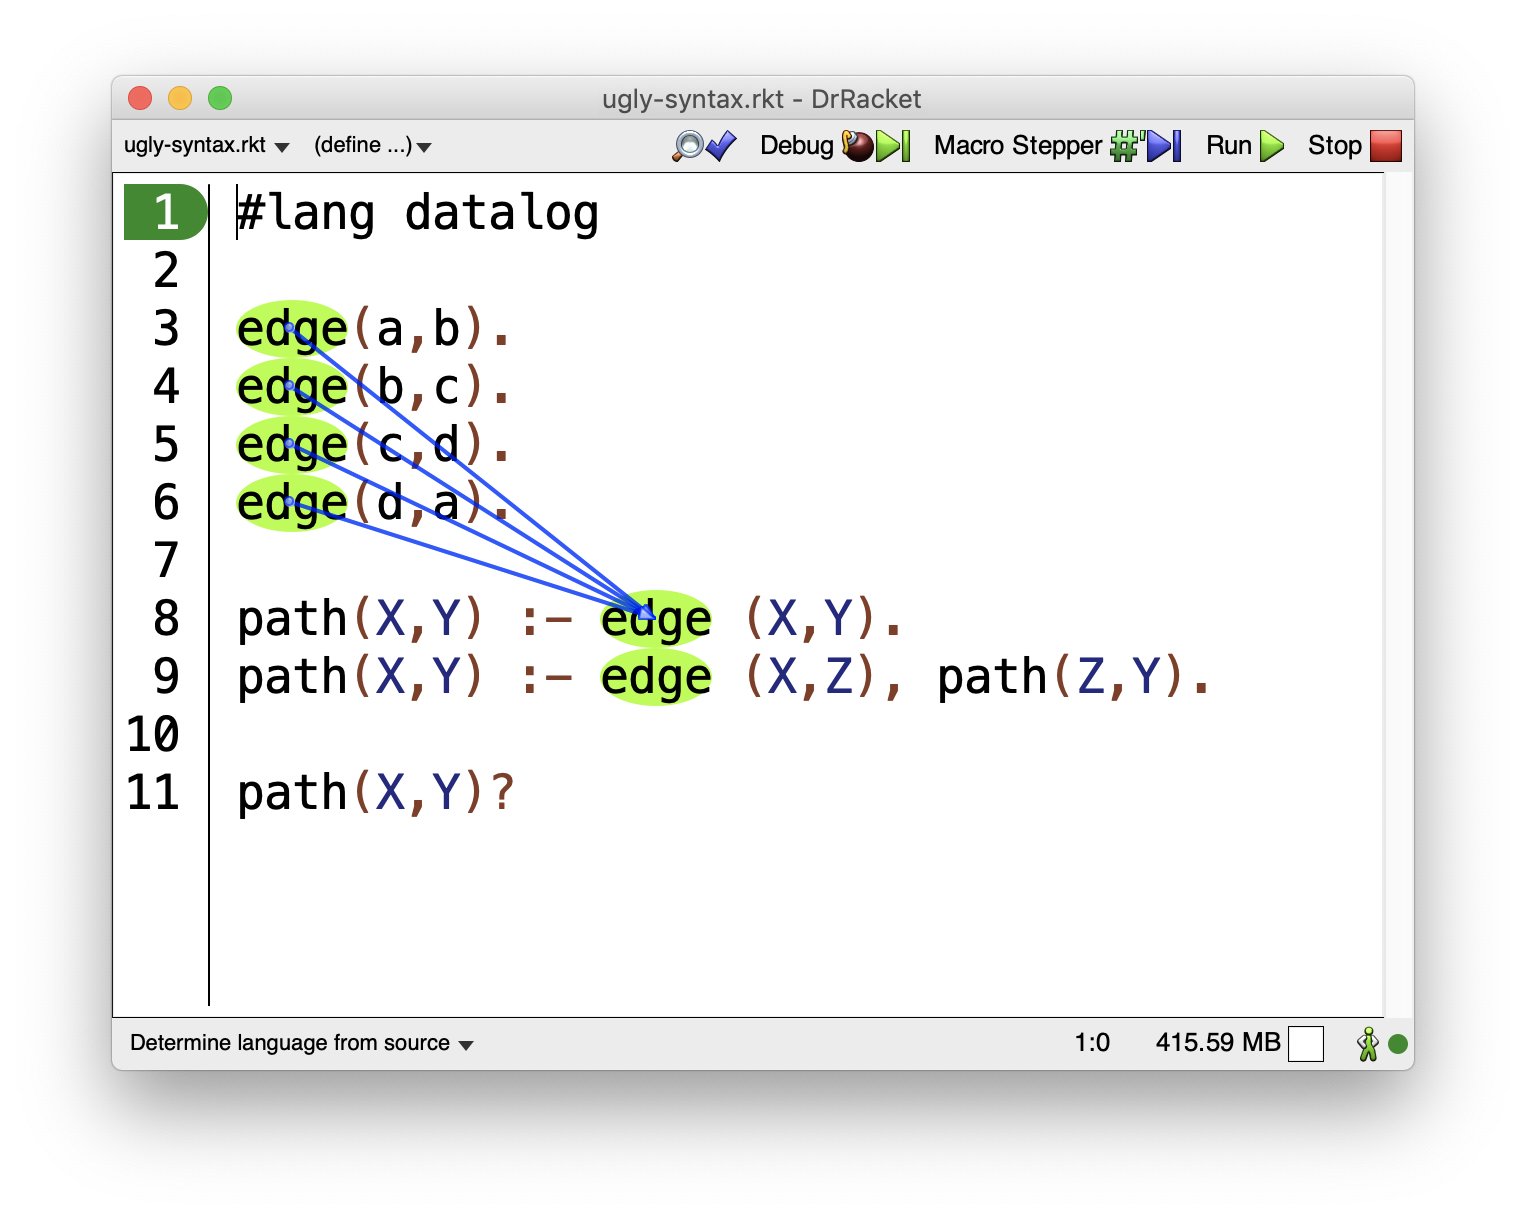
\includegraphics[]{images/racket-variable-arrow.png}
    \end{adjustbox}
    \caption{Результат интеграции языка datalog в IDE DrRacket.}\label{fig:racket-variable-arrow}
\end{figure}


\subsubsection{Структура программы}\label{sec:ch2/sec1/sub1/sub1}

Структура программы-описания аппаратного обеспечения имеет следующий вид, рисунок \ref{fig:device-program-structure}.

\begin{figure}[!htbp]
    \centering
    % !TEX encoding = UTF-8 Unicode
% Úτƒ-8 encoded
% http://www.linux.org.ru/forum/general/10357036
\tikzset{
    line/.style={draw, -latex'},
    every join/.style={line},
    u/.style={anchor=south},
    r/.style={anchor=west},
    fxd/.style={text width = 6em},
    it/.style={font={\small\itshape}},
    bf/.style={font={\small\bfseries}},
}
\tikzstyle{base_long} =
    [
        draw,
        on chain,
        on grid,
        align=center,
        minimum height=4ex,
        minimum width = 10ex,
        node distance = 6mm and 60mm,
        text badly centered,
    ]
\tikzstyle{base} =
    [
        draw,
        on chain,
        on grid,
        align=center,
        minimum height=4ex,
        minimum width = 10ex,
        node distance = 6mm and 60mm,
        text badly centered,
        text width=5cm
    ]
\tikzstyle{coord} =
    [
        coordinate,
        on chain,
        on grid
    ]
\tikzstyle{cloud} =
    [
        base,
        ellipse,
        node distance = 3cm,
        minimum height = 2em,
        text width=2cm
    ]
\tikzstyle{decision} =
    [
        base,
        diamond,
        aspect=2,
        node distance = 2cm,
        inner sep = 0pt
    ]
\tikzstyle{block} =
    [
        rectangle,
        base,
        rounded corners,
        minimum height = 2em
    ]
\tikzstyle{print_block} =
    [
        base,
        tape,
        tape bend top=none,
    ]
\tikzstyle{io} =
    [
        base,
        trapezium,
        trapezium left angle = 70,
        trapezium right angle = 110,
    ]
\tikzstyle{prompt} =
    [
        base,
        trapezium,
        trapezium left angle = 90,
        trapezium right angle = 80,
        shape border rotate = 90
    ]
\tikzstyle{disk file} =
    [
        base,
        cylinder,
        aspect=0.2,
    ]
\tikzstyle{process} =
    [
        rectangle,
        base,
    ]
\makeatletter
\pgfkeys{/pgf/.cd,
    subrtshape w/.initial=2mm,
    cycleshape w/.initial=2mm
}
\pgfdeclareshape{parallelshape}{
    \inheritsavedanchors[from=rectangle]
    \inheritanchorborder[from=rectangle]
    \inheritanchor[from=rectangle]{north}
    \inheritanchor[from=rectangle]{center}
    \inheritanchor[from=rectangle]{west}
    \inheritanchor[from=rectangle]{east}
    \inheritanchor[from=rectangle]{mid}
    \inheritanchor[from=rectangle]{base}
    \inheritanchor[from=rectangle]{south}
    \backgroundpath{
        \southwest \pgf@xa=\pgf@x \pgf@ya=\pgf@y
        \northeast \pgf@xb=\pgf@x \pgf@yb=\pgf@y
        \def\ppd@offset{\pgfpoint{\pgfutil@tempdima}{0ex}}
        \def\ppd@offsetm{\pgfpoint{-\pgfutil@tempdima}{0ex}}
        \pgfpathmoveto{\pgfqpoint{\pgf@xa}{\pgf@ya}}
            \pgfpathlineto{\pgfqpoint{\pgf@xb}{\pgf@ya}}
        \pgfpathclose
        \pgfpathmoveto{\pgfqpoint{\pgf@xb}{\pgf@yb}}
            \pgfpathlineto{\pgfqpoint{\pgf@xa}{\pgf@yb}}
        \pgfpathclose
    }
}
\pgfdeclareshape{subrtshape}{
    \inheritsavedanchors[from=rectangle]
    \inheritanchorborder[from=rectangle]
    \inheritanchor[from=rectangle]{north}
    \inheritanchor[from=rectangle]{center}
    \inheritanchor[from=rectangle]{west}
    \inheritanchor[from=rectangle]{east}
    \inheritanchor[from=rectangle]{mid}
    \inheritanchor[from=rectangle]{base}
    \inheritanchor[from=rectangle]{south}
    \backgroundpath{
        \southwest \pgf@xa=\pgf@x \pgf@ya=\pgf@y
        \northeast \pgf@xb=\pgf@x \pgf@yb=\pgf@y
        \pgfmathsetlength\pgfutil@tempdima{\pgfkeysvalueof{/pgf/subrtshape w}}
        \def\ppd@offset{\pgfpoint{\pgfutil@tempdima}{0ex}}
        \def\ppd@offsetm{\pgfpoint{-\pgfutil@tempdima}{0ex}}
        \pgfpathmoveto{\pgfqpoint{\pgf@xa}{\pgf@ya}}
        \pgfpathlineto{\pgfqpoint{\pgf@xb}{\pgf@ya}}
        \pgfpathlineto{\pgfqpoint{\pgf@xb}{\pgf@yb}}
        \pgfpathlineto{\pgfqpoint{\pgf@xa}{\pgf@yb}}
        \pgfpathclose
        \pgfpathmoveto{\pgfpointadd{\pgfpoint{\pgf@xa}{\pgf@yb}}{\ppd@offsetm}}
        \pgfpathlineto{\pgfpointadd{\pgfpoint{\pgf@xa}{\pgf@ya}}{\ppd@offsetm}}
        \pgfpathlineto{\pgfpointadd{\pgfpoint{\pgf@xb}{\pgf@ya}}{\ppd@offset}}
        \pgfpathlineto{\pgfpointadd{\pgfpoint{\pgf@xb}{\pgf@yb}}{\ppd@offset}}
        \pgfpathclose
    }
}
\pgfdeclareshape{cyclebegshape}{
    \inheritsavedanchors[from=rectangle]
    \inheritanchorborder[from=rectangle]
    \inheritanchor[from=rectangle]{north}
    \inheritanchor[from=rectangle]{center}
    \inheritanchor[from=rectangle]{west}
    \inheritanchor[from=rectangle]{east}
    \inheritanchor[from=rectangle]{mid}
    \inheritanchor[from=rectangle]{base}
    \inheritanchor[from=rectangle]{south}
    \backgroundpath{
        \southwest \pgf@xa=\pgf@x \pgf@ya=\pgf@y
        \northeast \pgf@xb=\pgf@x \pgf@yb=\pgf@y
        \pgfmathsetlength\pgfutil@tempdima{\pgfkeysvalueof{/pgf/cycleshape w}}
        \pgfpathmoveto{\pgfqpoint{\pgf@xa}{\pgf@ya}}
\pgfpathlineto{\pgfpointadd{\pgfpoint{\pgf@xa}{\pgf@yb}}{\pgfpoint{0ex}{-\pgfutil@tempdima}}}
\pgfpathlineto{\pgfpointadd{\pgfpoint{\pgf@xa}{\pgf@yb}}{\pgfpoint{\pgfutil@tempdima}{0ex}}}
\pgfpathlineto{\pgfpointadd{\pgfpoint{\pgf@xb}{\pgf@yb}}{\pgfpoint{-\pgfutil@tempdima}{0ex}}}
\pgfpathlineto{\pgfpointadd{\pgfpoint{\pgf@xb}{\pgf@yb}}{\pgfpoint{0ex}{-\pgfutil@tempdima}}}
\pgfpathlineto{\pgfqpoint{\pgf@xb}{\pgf@ya}}
        \pgfpathclose
    }
}
\pgfdeclareshape{cycleendshape}{
    \inheritsavedanchors[from=rectangle]
    \inheritanchorborder[from=rectangle]
    \inheritanchor[from=rectangle]{north}
    \inheritanchor[from=rectangle]{center}
    \inheritanchor[from=rectangle]{west}
    \inheritanchor[from=rectangle]{east}
    \inheritanchor[from=rectangle]{mid}
    \inheritanchor[from=rectangle]{base}
    \inheritanchor[from=rectangle]{south}
    \backgroundpath{
        \southwest \pgf@xa=\pgf@x \pgf@ya=\pgf@y
        \northeast \pgf@xb=\pgf@x \pgf@yb=\pgf@y
        \pgfmathsetlength\pgfutil@tempdima{\pgfkeysvalueof{/pgf/cycleshape w}}
        \pgfpathmoveto{\pgfqpoint{\pgf@xb}{\pgf@yb}}
\pgfpathlineto{\pgfpointadd{\pgfpoint{\pgf@xb}{\pgf@ya}}{\pgfpoint{0ex}{\pgfutil@tempdima}}}
\pgfpathlineto{\pgfpointadd{\pgfpoint{\pgf@xb}{\pgf@ya}}{\pgfpoint{-\pgfutil@tempdima}{0ex}}}
\pgfpathlineto{\pgfpointadd{\pgfpoint{\pgf@xa}{\pgf@ya}}{\pgfpoint{\pgfutil@tempdima}{0ex}}}
\pgfpathlineto{\pgfpointadd{\pgfpoint{\pgf@xa}{\pgf@ya}}{\pgfpoint{0ex}{\pgfutil@tempdima}}}
\pgfpathlineto{\pgfqpoint{\pgf@xa}{\pgf@yb}}
        \pgfpathclose
    }
}
\makeatother
\tikzstyle{subroutine} =
    [
        base,
        subrtshape,
    ]
\tikzstyle{cyclebegin} =
    [
        base,
        cyclebegshape,
    ]
\tikzstyle{cycleend} =
    [
        base,
        cycleendshape,
    ]
\tikzstyle{connector} =
    [
        base,
        circle,
    ]

\tikzstyle{parallel} =
    [
        base_long,
        parallelshape,
    ]
\begin{tikzpicture}[%
    start chain=going below,    % General flow is top-to-bottom
    node distance=6mm and 30mm, % Global setup of box spacing
    ]
        \node  [rectangle,
                base,
                minimum width=6cm] (device class)
                {Описание класса устройства};
        \node  [rectangle,
                base,
                minimum width=6cm] (c-python api)
                [below = 1.5cm of device class]
                {Связывание функций C-Python интерфейса};
        \node  [rectangle,
                base,
                minimum width=6cm] (py logic)
                [below = 1.85cm of c-python api]
                {Реализация логики работы устройства на Python};



\end{tikzpicture}

    \caption{Структура программы-описания аппаратного обеспечения.}\label{fig:device-program-structure}
\end{figure}

Несмотря на то, что компилятор язык программы-описания располагает
блоки кода в результирующем тексте модуле QEMU в соответствии
с правилами языка C и порядок объявления блоков в исходном файле ему не важен,
данная структура является наиболее понятной и органичной для стороннего разработчика.
Поэтому компилятор принуждает программиста придерживаться её, подобно тому, как
язык Python обязывает использовать отступы для создания блоков кода.


\subsubsection{Граммматика языка}\label{sec:ch2/sec1/sub1/sub2}
Разрабатываемый язык является языком с контекстно-свободной грамматикой.
Далее он будет именоваться как {\mylanguage} (произносится \mylanguageprononciation)

Грамматика {\mylanguage} ограничена до описания зависимостей устройства и QEMU,
связывания функций C и Python, встраивания Python-кода с логикой работы устройства
в файл.


% TODO: Учтено ли, что пользователь захочет кастомизировать функции инициализации класса и инстанса?
% TODO: MemoryRegionOps?
\setlength{\grammarparsep}{0.1cm}
\setlength{\grammarindent}{13em}
\begin{figure}[!htbp]
    \begin{grammar}
        <letter> ::= `a' ... `z' | `A' ... `Z';

        <digit> ::= `0' ... `9' ;

        <symbol> ::= \symbol{92}x20 ... \symbol{92}x7E ; (* любой печатный символ, согласно кодам ASCII *)

        <const value> ::= <digit> | `"' \{ <symbol> \} `"';

        <identifier> ::= <letter> [\{ <letter> | <digit> | `\_' \}] ;

        <block start> ::= `{';

        <block end> ::= `}';

        <field> ::= <identifier> `=' <identifier> | <block> ;

        <block> ::= <block start> <field> [\{ `,' <field> \}] <block end>;

        <device definition> ::= '\#' <identifier>;

        <device class inheritance> ::= `(' <identifier> `:' <identifier> [\{ `,' <identifier> \}] `)';

        <device class block> ::= <device class inheritance> <block>;

        <bind block> ::= `@bind' <block>;

        <python block> ::= `@py' <block>;

        <program> ::= <device definition> <device class block> <bind block> <python block>;
    \end{grammar}
    \caption{Расширенная форма Бэкуса-Наура \mylanguage}\label{fig:qpydev-grammar}
\end{figure}


\subsubsection{Семантика языка}\label{sec:ch2/sec1/sub1/sub3}

Для описания семантики языка {\mylanguage} была выбрана денотационная семантика.
Краеугольным камнем денотационной семантики является определение для каждой сущности
языка некоего математического объекта и некоей функции, называемой интерпретатором,
которая отображает экземпляры этой сущности в экземпляры этого математического объекта -- элемент множества денотаций.
Поскольку математические объекты строго определены, то они представляют собой точный
смысл соответствующих сущностей.

Функции обозначают посредством двойных квадратных скобок $[[$ $]]$,
а элемент алгебры или операция алгебры, сопоставленные функцией $[[$ $]]$
правильному выражению или конструктору выражений, называют денотантом этого выражения или,
соответственно, денотацией конструкции. \cite{denotational-semantics}

Для языка {\mylanguage} значимыми множествами семантических объектов
являются только множества $Q$ -- объектов QEMU (переменные, функции, структуры) и
$C$ -- множество константных выражений.


\begin{figure}[!htbp]
    \centering
    \begingroup
    \addtolength{\jot}{1em}
    \begin{align*}
        [[assignment]](x,y) ={}& \lambda x.y \\
        [[terminate]](m) ={}& \text{ Завершение работы компилятора} \\
        [[if]](c,e_1,e_2) ={}&
        \begin{cases}
            e_1, & \text{Если } c = true \\
            e_2, & \text{Если } c \not= true
        \end{cases} \\
        [[throw\ error]](c, e) ={}& if(c, e_g, terminate) \\
        [[lookup]](o) ={}& [[throw\ error]](o \in Q, o) \\
        [[<device\ definition>]](i) ={}& lookup(i) \\
        [[<device\ class\ inheritance>]](i_1,...,i_n) ={}& lookup(i_1) + ... + lookup(i_n) \\
        [[<field>]](v_1, v_2) ={}& assignment(v_1, v_2),\\ & \text{ Если } v_1 \in Q \text{ и } v_3 \in C \cup Q \\
        [[<block>]](f_1,...,f_n) ={}& field(f_1) + ... + field(f_n) \\
        [[<python block>]](b) ={}& assignment(B,B)\\
    \end{align*}
    \endgroup
    \caption{Денотационная семантика {\mylanguage}}\label{fig:denotational-semantics}
\end{figure}


\subsection{Поиск используемых сущностей QEMU}\label{sec:ch2/sec1/sub2}

Пробрасывание -- процесс преобразовывания и передачи данных между двумя интерфейсами.

Поиск используемых сущностей состоит в установлении типов QEMU для последующего
корректного пробрасывания их в логику устройства.
Также это необходимо для проверки корректности наследования и встраивания устройства.
Необходимыми для пробрасывания типами являются структуры и функции, оперирующие ими.

Рекурсивное преобразование структур QEMU в типы python важно для удобного и читаемого
использования C-объектов внутри python-логики.
Пробрасывание в python функций QEMU необходимо для использования уже имеющегося API эмулятора.
% TODO: может удалить, если это сложно
Потенциально, может быть удобным использование макросов препроцессора C внутри
логики Python.

Базовым классом для всех классов QEMU является класс \texttt{Object}.
Наследование происходит через определение первым членом C-структуры
указателя на структуру-родитель данной. Так как язык C гарантирует, что
первый член структуры всегда начинается с нулевого отступа от начала
структуры, любой класс можно привести к типу Object.
В свою очередь Object содержит структуру, описывающую класс приведенного
объекта -- \texttt{ObjectClass}, что позволяет определить реальный тип указателя
во время исполнения.

Структуры \texttt{TypeImpl} и \texttt{TypeInfo} (см рис. \ref{fig:qom-structure}) практически не отличаются,
но служат для разных целей:
\texttt{TypeImpl} является <<внутренним>> содержанием класса, служебной структурой,
которая скрывает методы класса от пользователя интерфейса, тогда как \texttt{TypeInfo}
наоборот, предоставляет уже очищенный от служебных полей интерфейс для инициализации \texttt{TypeImpl}.

После объявления \texttt{TypeInfo}, структура регистрируется в объектной системе QEMU.
Это происходит через использование макроса \texttt{type\_init}, который создает, можно считать,
анонимную функцию, в свою очередь вызывающую функцию \texttt{register\_module\_init}.
Созданная анонимная функция помечается атрибутом \texttt{constructor} \cite{gcc-attributes}, что заставляет
компилятор добавить вызов такой функции до вызова функции main.
Соответственно, инициализация модулей происходит до того, как начнет исполняться логика QEMU.

% TODO: А точно ли?

Все перефирийные устройства, добавляемые в QEMU, <<общаются>> с другими устройствами через чтение и запись
по определенным для устройства адресам памяти.
За это отвечает структура \texttt{MemoryRegionOps} \ref{fig:mem-reg-ops},
которая инициализируется функциями чтения и записи,
которые вызываются, соответственно, при чтении или записи памяти, на которое <отображено>> устройство.
Данные функции принимают на вход указатель на устройство, в чью память происходит чтение или запись,
адрес, по которому происходит чтение или запись, и, в случае чтения, количество читаемых байт,
а в случае записи -- записываемое значение и количество записываемых байт.
Некоторые устройства используют расширенные версии чтения и записи, где последним аргументом передается
структура с атрибутами транзакции.

\begin{figure}[!htbp]
    \centering
    \begin{adjustbox}{max totalsize={\textwidth}{\textheight}}
        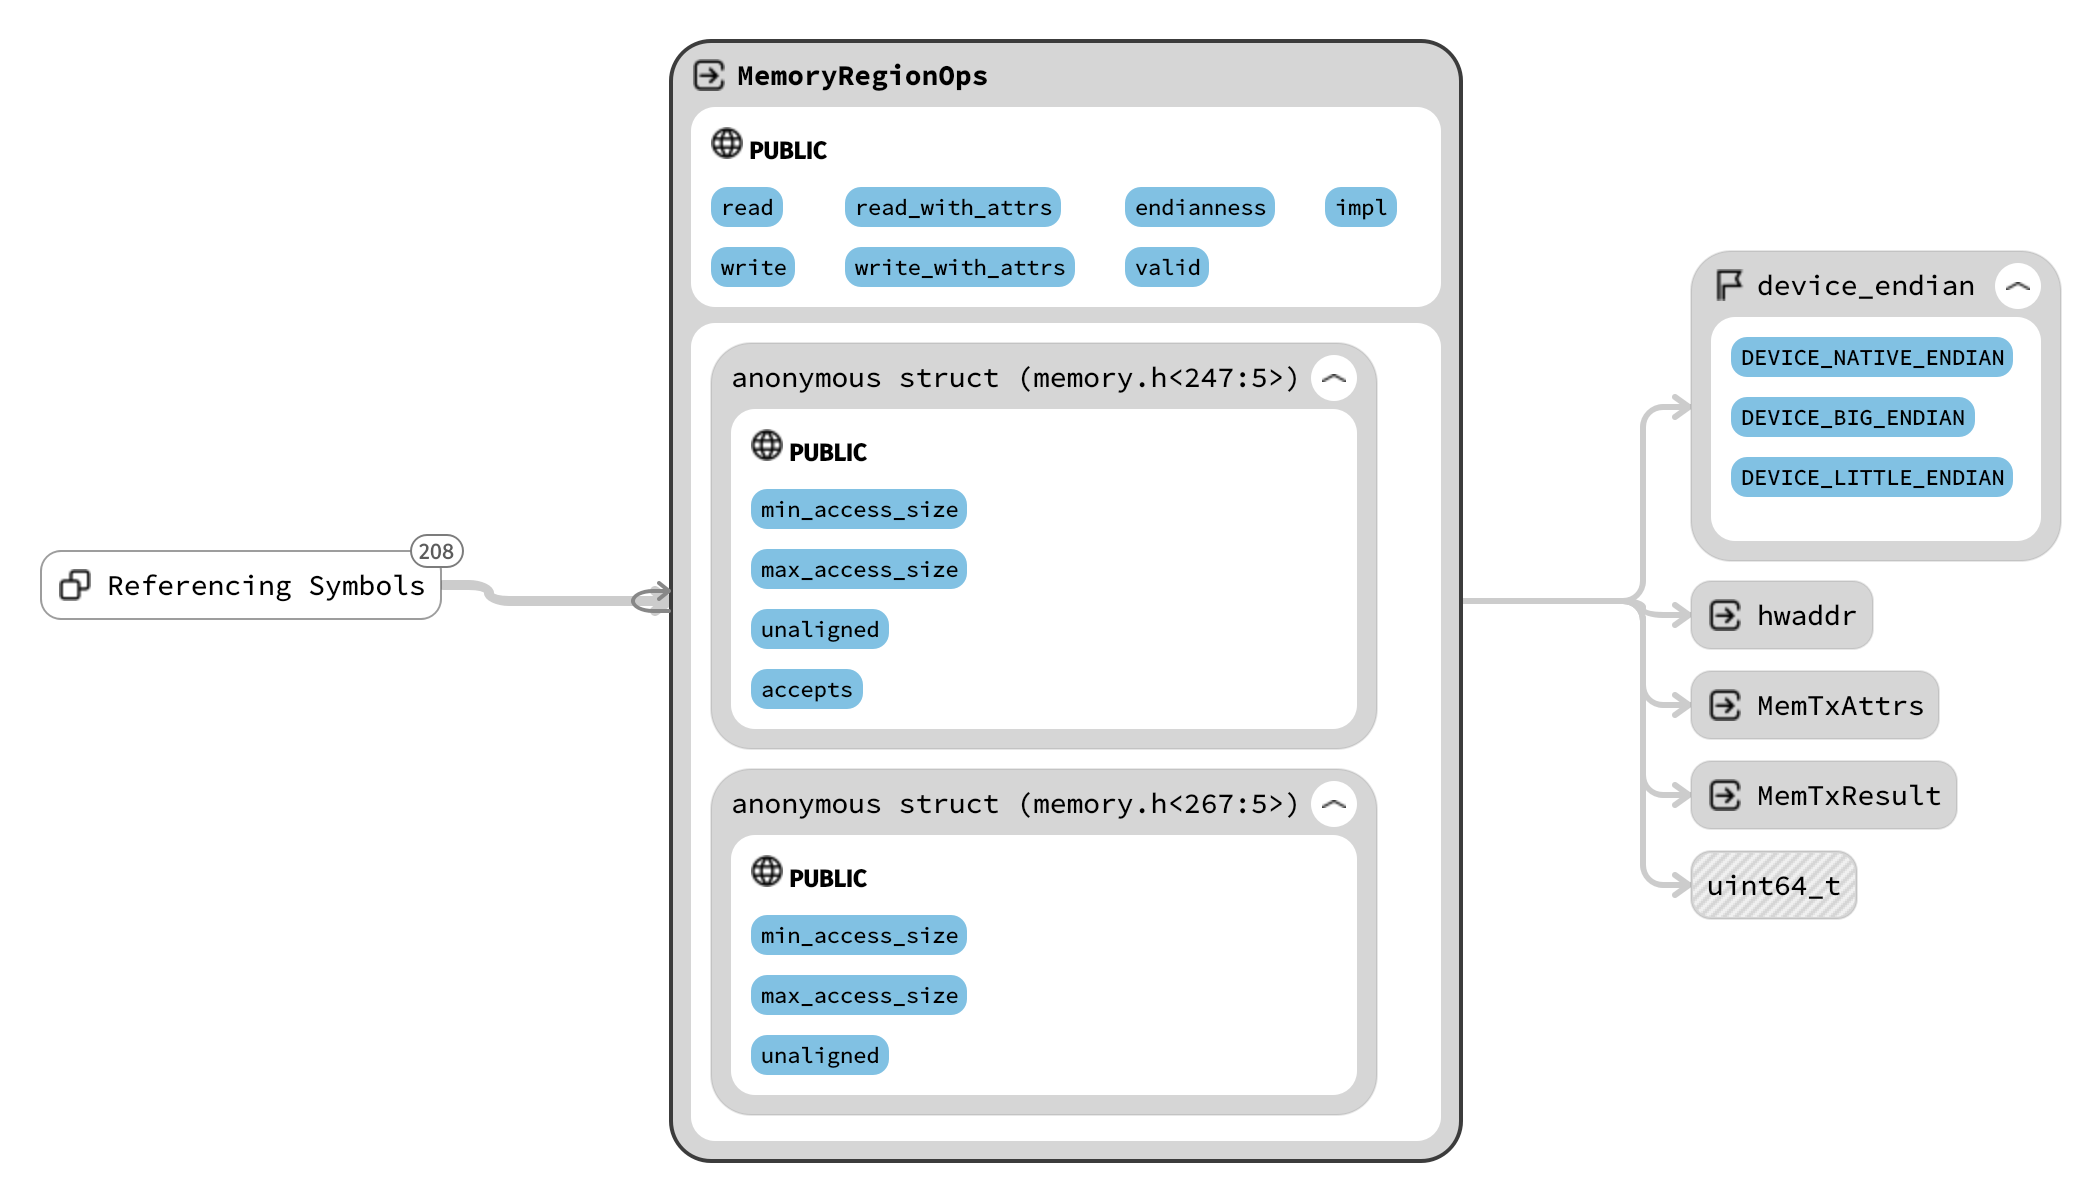
\includegraphics[]{images/mem_reg_ops_cropped.png}
    \end{adjustbox}
    \caption{Связь \texttt{MemoryRegionOps} с другими сущностями QEMU.}\label{fig:mem-reg-ops}
\end{figure}


\subsubsection{Механизм нахождения информации о типах устройств}\label{sec:ch2/sec1/sub2/sub1}

Все устройства QEMU:
\begin{enumerate}[label={\arabic*)}]
    \item имеют родителя и распределены по подпапкам папки \texttt{hw};
    \item объявляют структуру \texttt{TypeInfo}, в которой указывается родитель устройства
          и размер создаваемого объекта -- поле \texttt{.instance\_size}
          (используется для создания объектов устройств на системной шине);
    \item используют оператор \texttt{sizeof},
          передавая ему имя структуры устройства, которое будет исполняться в QEMU.
\end{enumerate}

Данная информация позволяет найти используемые сущности QEMU следующим образом:
\begin{enumerate}[label={\arabic*)}]
    \item пройтись по всем файлам, находящимся в папке \texttt{hw};
    \begin{enumerate}[label={\arabic*)}]
        \item найти структуру \texttt{TypeInfo};
        \item проанализировать поле \texttt{.instance\_size} и сохранить
              используемую структуру как возможную для наследования;
        \item сохранить поле \texttt{.name} в качестве имени структуры для наследования;
    \end{enumerate}
\end{enumerate}

Помимо явного описания структуры \texttt{TypeInfo} некоторые устройства, написанные
в современном стиле, используют макросы:
\begin{enumerate}[label={\arabic*)}]
    \item \label{main-def-macro} \texttt{OBJECT\_DEFINE\_TYPE\_EXTENDED};
    \item \texttt{OBJECT\_DEFINE\_TYPE};
    \item \texttt{OBJECT\_DEFINE\_TYPE\_WITH\_INTERFACES};
    \item \texttt{OBJECT\_DEFINE\_ABSTRACT\_TYPE}.
\end{enumerate}

Все перечисленные макросы создают структуру \texttt{TypeInfo} и все, кроме \ref{main-def-macro},
вызывают внутри себя макрос \ref{main-def-macro}, специализируя определенные поля структуры \texttt{TypeInfo}.
Например \texttt{OBJECT\_DEFINE\_ABSTRACT\_TYPE} создает абстрактный тип, передавая внутри себя
значение \texttt{true} макросу \texttt{OBJECT\_DEFINE\_TYPE\_EXTENDED}, чем облегчает собственный интерфейс
и делает свое использование более выразительным.

Список аргументов макросов объявления типов также требуется разбирать, чтобы получить из аргументов информацию
о структуре \texttt{TypeInfo}.

Механизм получения информации о функциях намного проще: в языке C функции могут инкапсулироваться
только на уровне одного модуля трансляции -- C-файла, прошедшего этап препроцессирования.
Инкапсулированные функции помечаются ключевым словом \texttt{static}, что делает их
<<невидимыми>> в других модулях трансляции.
Все функции, не помеченные ключевым словом \texttt{static} будем считать интерфейсными.

Данная информация будет использована впоследствии для корректной кодогенерации устройства
и преобразования C-структур и C-функций в читаемый вид для python-интерфейса.

\subsubsection{Механизм использования информации о типах устройств}\label{sec:ch2/sec1/sub2/sub2}

Так как код QEMU насыщен использованием макросов, потребуется инструмент для их разворачивания -- препроцессор.
Чтобы не создавать собственную имплементацию препроцессора, этим будет заниматься препоцессор системного компилятора.

Практически во всех системах сборки программ в POSIX окружении используется компилятор gcc или clang.
Оба компилятора являются совместимыми между собой. Для задействования препроцессора компилятора используется
опция \texttt{-E}. Так как препроцессор C, помимо раскрытия макросв занимается еще нахождением и подстановкой
заголовочных файлов, то потребуется указать папки с их местонахождением.
QEMU полагается на:
\begin{enumerate}[label={\arabic*)}]
    \item \label{build-header} заголовочные файлы, создаваемые в процессе сборки эмулятора;
    \item библиотеку GLib;
    \item заголовочные файлы, находящиеся в папке \texttt{include}.
\end{enumerate}

Так как файлы в пункте \ref{build-header} появляются в процессе сборки, то конкретную версию QEMU нужно будет собрать.
Сборка также полезна, так как в процессе конфигурации эмулятора выставляются определенные переменные
препроцессора (дефайны -- от директивы \texttt{\#define}), которые влияют на условные выражения
препроцессора, а те, в свою очередь, на генерацию исходного кода.
Использование в данном случае статического анализатора кода было бы затруднительным, так как
информация о конкретной конфигурации не может быть получена без непосредственной сборки.

Укзание папки для препроцессора производится с помощью опции \texttt{-I}.
\begin{lstlisting}[caption={Пример строки запуска препроцессора для определенного файла устройства},
                   captionpos=b]
gcc -E hw/misc/edu.c
    -I ./include/
    -I ./build/
    -I/usr/include/glib-2.0
    -I/usr/lib64/glib-2.0/include
\end{lstlisting}


\subsection{Генерация python-интерфейса для логики устройства}\label{sec:ch2/sec1/sub3}

% TODO: как это вяжется со SWIG'ом?
Определение интерфейса используемых сущностей QEMU происходит в уже препроцессированном коде \ref{sec:ch2/sec1/sub2/sub2}.

\subsubsection{Генерация python-интерфейса для C-кода}\label{sec:ch2/sec1/sub3/sub1}

Язык Python является скорее интерфейсом, чем языком программирования:
документация описывает то, какие функции и конструкции должен предоставлять язык, чтобы являться Python'ом.
Подтверждением этому служит большое количество различных реализаций языка, например:
\begin{itemize}
    \item IronPython/Jython -- интерпретатор, работающий в CLR и JVM соответственно;
    \item PyPy -- JIT-интерпретатор, изначально написанный на самом Python;
    \item CPython -- эталонный интерпретатор Python, написанный на языке C;
\end{itemize}

Под языком Python практически всегда понимается интерпретатор CPython, как раз его
API для создания связки между кодом на C и Python и будет использоваться.

Для создания бесшовной интеграции, требуется:
\begin{itemize}
    \item преобразовывать C-структуры и C-функции в Python-объекты;
    \item оборачивать C-функции для конвертации Python-аргументов в C-типы;
    \item транслировать изменения связанных объектов внутри Python-кода.
\end{itemize}

\paragraph{SWIG} --  Simplified Wrapper and Interface Generator.
Данное ПО позволяет автоматически генерировать обертки над C/C++ библиотеками для
большого спектра высокоуровневых языков программирования (рис. \ref{fig:swig}).
Для этого требуется написать интерфейсный файл, в котором будут описаны шаблоны
функций и структур, для которых требуется сгенерировать интерфейс.
SWIG принимает на вход файл с описанием шаблонов для нахождения структур и
функций, которые будут экспортированы в межъязыковой интерфейс.
Не смотря на удобство, SWIG не обладает возможностями препроцессора и понимает
только ограниченное количество его директив, причем \texttt{define}'ы воспринимает
только если они объявляют константы.

\begin{figure}[!htbp]
    \centering
    \begin{adjustbox}{max totalsize={\textwidth}{\textheight}}
        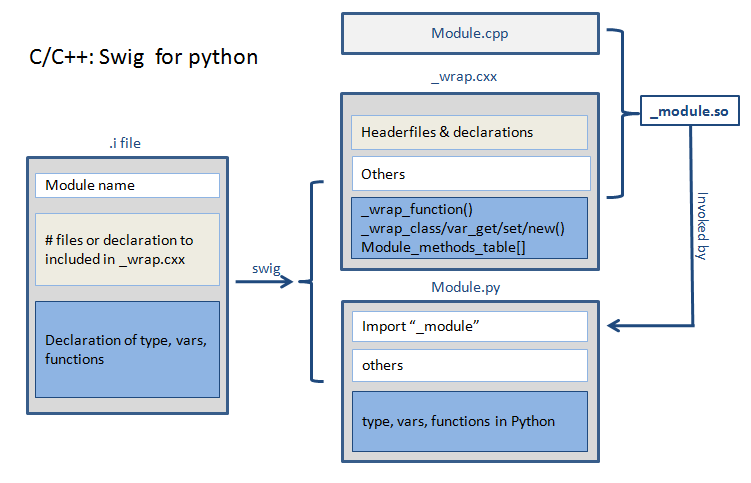
\includegraphics[]{images/swig.png}
    \end{adjustbox}
    \caption{Схема работы SWIG.}\label{fig:swig}
\end{figure}

Исходя из этого и того, что SWIG генерирует очень большое количество кода,
который все равно придется дополнять обращениями к C-API Python то логичнее
реализовать свое нахождение и преобразование C-сущностей.

В Python существует несколько способов импорта C-сущностей:

\begin{enumerate}[label={\arabic*)}]
    \item \texttt{PyCapsule} -- позволяет инкапсулировать и передавать данные, находящиеся по некому указателю
          сквозь Python-код обратно в C. Сам Python не имеет доступа к инкапсулированному объекту
          так как не сохраняет никакой информации о типе. Ограничением в использовании \texttt{PyCapsule}
          является невозможность работы с данным объектом из многопоточного кода, так как
          Python не может его сериализовать;
    \item \texttt{memoryview} -- созданные объекты являются <<отображениями>> памяти, дают доступ
          к некоторому C-буферу, обозначенному при создании объекта. Можно использовать для
          экспорта сущностей, но с перекладыванием ответственности на интерпретацию байтов буфера
          на Python-код;
    \item Создание Python-объекта, отражающего C-сущность. Можно выполнить отдельным классом или
          же словарем.
\end{enumerate}

В {\mylanguage} для C-сущностей генерируются классы, отражающие их внутреннее устройство.
Объекты классов не имеют полей, и могут быть использованы только через оператор \texttt{[]}.
В пардигме Python, данный оператор является <<синтаксическим сахаром>> для вызова <<магических>>
функций \texttt{\_\_setitem\_\_} для выставления поля и \texttt{\_\_getitem\_\_} для получения значения.
В данном случае для \texttt{\_\_setitem\_\_} и \texttt{\_\_getitem\_\_} согласно C-API \cite{python-c-type-objects}
генерируются функции, которые первым делом производят конвертацию Python-типов в C-типы, после чего
уже возвращают или выставляют сконвертированные значения в структуры (листинг \ref{lst:python-c-type-objects}).


\begin{lstlisting}[caption={Пример доступа к элементу структуры из Python.},
                   captionpos=b,
                   language=python]
# вызывается функция __getitem__, которая по возможности
# конвертирует C-тип в Python-тип и возвращает Python-сущность,
# присваивая её переменной source.
source = EduState["dma_state"]["src"]

# вызывается функция __setitem__, которая по возможности
# конвертирует Python-тип в C-тип, после чего
# полю EduState.dma_state.dst присваивается значение.
EduState["dma_state"]["dst"] = source + 0x1234
\end{lstlisting}\label{lst:python-c-type-objects}

% TODO: Учтено ли, что пользователь захочет кастомизировать функции инициализации класса и инстанса?
Python-интерфейс 

\subsection{Генерация C-интерфейса устройства в QEMU}\label{sec:ch2/sec1/sub4}

\subsection{Проброс ошибок QEMU из и в Python}\label{sec:ch2/sec1/sub5}
\subsection{Встраивание устройства в сборку QEMU}\label{sec:ch2/sec1/sub6}
\subsection{Сборка QEMU}\label{sec:ch2/sec1/sub7}
